\documentclass[12pt, a4paper]{article}


\usepackage{wrapfig}
\usepackage{graphicx}
\usepackage[T1]{fontenc}
\usepackage[polish]{babel}
\usepackage[utf8]{inputenc}
\usepackage[font=footnotesize, labelfont=bf]{caption}
\usepackage{csquotes}
\usepackage{placeins}


\usepackage[backend=biber, sorting=ynt]{biblatex}
\addbibresource{draft.bib}

\newcommand{\code}[1]{\texttt{#1}}


\title{Bibliography
management:
\texttt{biblatex}
package}


\author{Krzytsztof
Wiśniewski}
\date{
}


\begin{document}
  \begin{titlepage}
    \centering


    \Large \textbf{UNIWERSYTET GDAŃSKI}\\ \textbf{WYDZIAŁ MATEMATYKI, FIZYKI I
    INFORMATYKI}

    \vspace{2.5cm}


    \large \textbf{Krzysztof Wiśniewski}\\ \textbf{numer albumu: 274276}

    \vspace{1.5cm}
    \raggedright \small Kierunek studiów: Bioinformatyka\\ Specjalność: Ogólna

    \vspace{1.5cm}


    \centering
    \Large \textbf{Optymalizacja oprogramowania w języku Python do analizy stanów kwantowych.}

    \vfill


    \raggedleft \normalsize Praca licencjacka\\ wykonana\\ pod kierunkiem\\ dr hab.
    Marcin Wieśniak, prof. UG\\

    \vfill


    \centering
    \large Gdańsk 2023
  \end{titlepage}
  \newpage


  \tableofcontents
  \newpage


  \begin{sloppypar}
    \begin{abstract}
      W tej pracy przeprowadzam analizę efektywności metod optymalizacji, która
      koncentruje się na minimalizacji czasu wykonania, oprogramowania napisanego w języku
      Python\cite{Python_Language}\cite{ML_Learning_Python}, skupiającego się na
      arytmetyce macierzowej, na przypadku programu CSSFinder służącego do analizy stanów
      kwantowych pod kątem detekcji splątania kwantowego. Pośród rozważanych metod
      obecna będzie standardowa implementacja w języku Python z wykorzystaniem
      biblioteki NumPy\cite{NumPy_Article}\cite{NumPy_Doc}, wersja wzbogacona o kompilację
      JIT przy pomocy biblioteki Numba\cite{Numba_Article}\cite{Numba_Doc}, wersja
      skompilowana do kodu maszynowego przy pomocy biblioteki Cython\cite{Cython_The_Best_Of_Both}\cite{Cython_Org}
      i kompilatora GCC\cite{GCC_Org} oraz implementacja w języku Rust\cite{Rust_Programming_Language},
      również skompilowana do kodu maszynowego.
    \end{abstract}

    \section{Wstęp}


    \subsection{Dlaczego Python?}


    Język Python zachęca użytkowników prostotą składni, łatwością tworzenia kodu,
    dynamicznym systemem typów, automatycznym zarządzanie pamięcią, mnogością dostępnych
    bibliotek otwartoźródłowych, oraz rozbudowaną społecznością programistów. Na
    przestrzeni ostatnich 20 lat język stworzony przez Guido van Rossum zanotował
    intensywny wzrost popularności. Pokazują to liczne zestawienia, w tym zestawienie
    najczęściej wykorzystywanych języków programowanie na GitHub'ie\cite{GitHub_Top_languages},
    w którym Python w roku 2022 zajął 2 miejsce, czy też zestawienie TIOBE Index\cite{TIOBE_Software_Index},
    uznające ten język za obecnie najbardziej rozpowszechniony pośród doświadczonych programistów
    (Maj 2023).

    \FloatBarrier
    \begin{figure}[h]
      \centering
      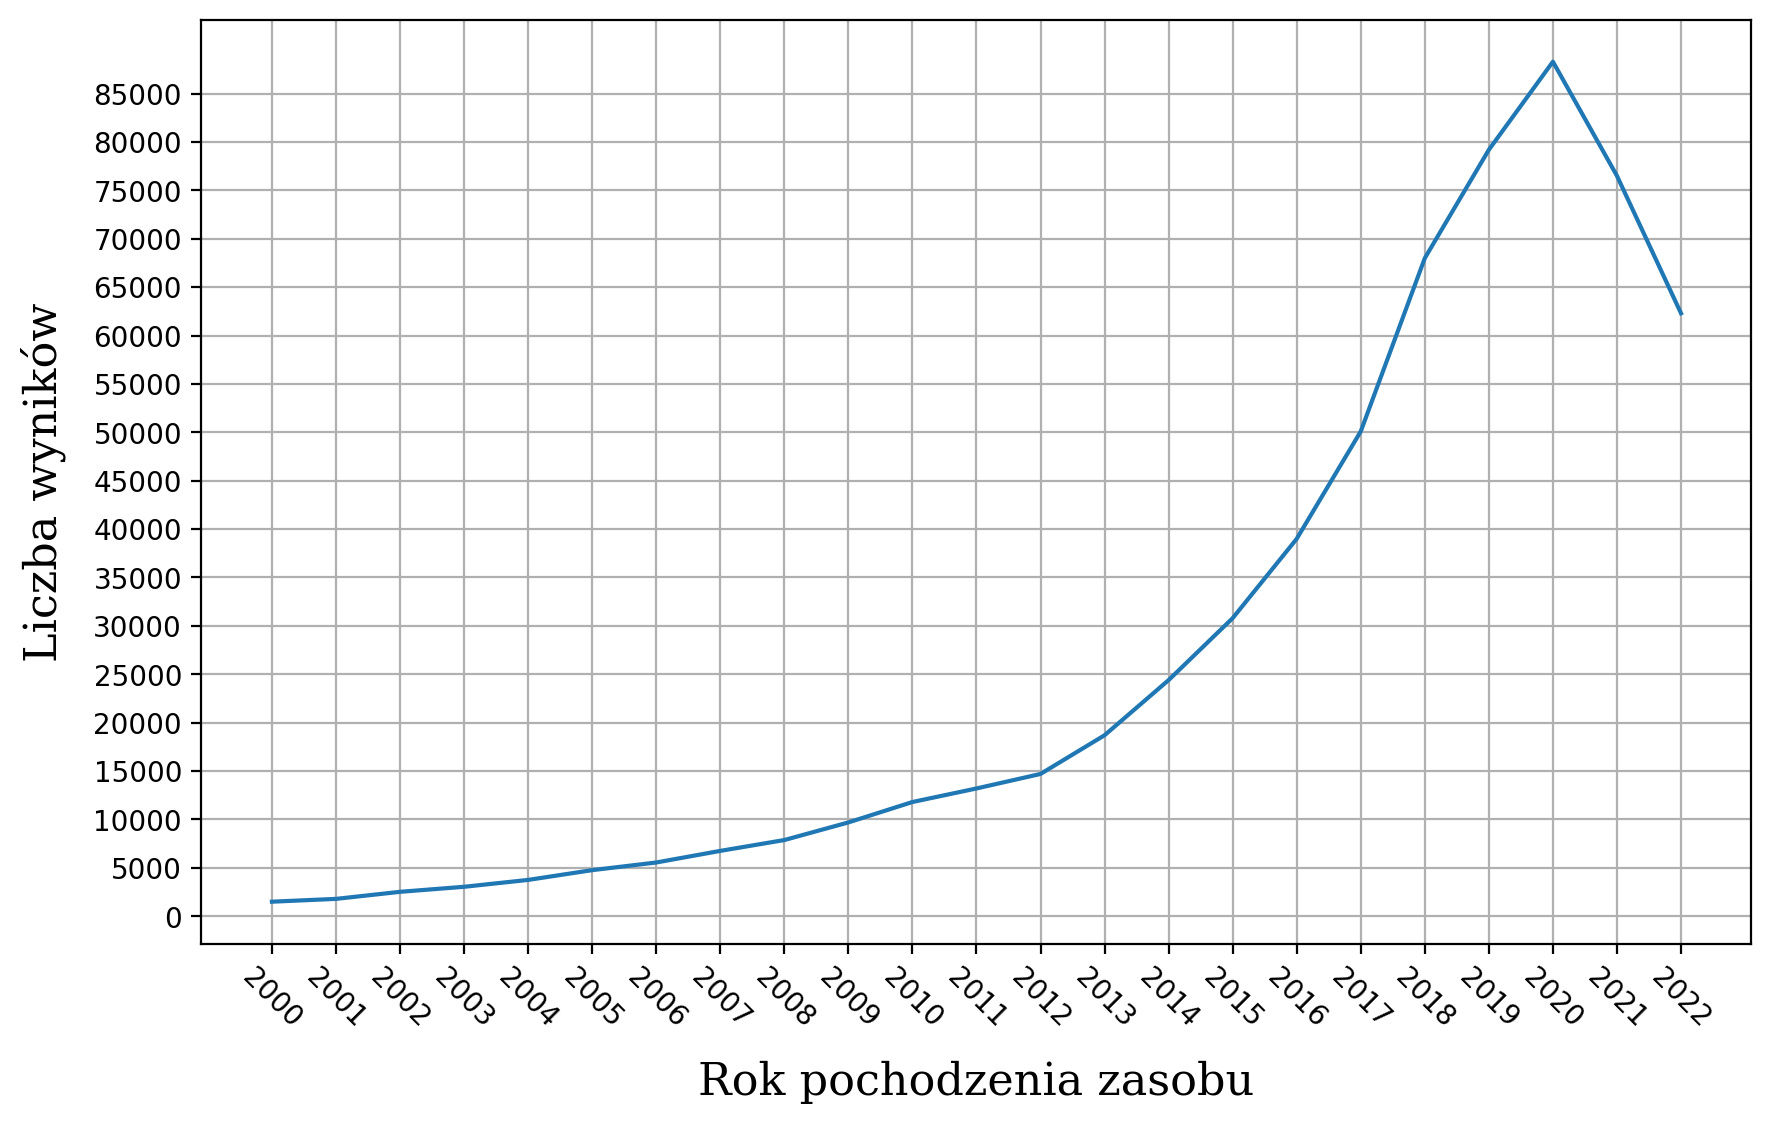
\includegraphics[width=0.75\textwidth]{"images/python_language_results.png"}
      \caption{Ilość wyników zwróconych przez wyszukiwarkę Google Scholar dla zapytania 'python language' z podziałem na rok wydania.}
    \end{figure}
    \FloatBarrier

    Niestety, interpretowany kod, napisany w Pythonie, pomimo licznych zalet, posiada
    również dotkliwą wadę - pod względem wydajności znacząco odstaje od kompilowanych
    języków programowania (C\cite{C_vs_Python}, C++\cite{Cpp_vs_Python}, Rust\cite{Rust_vs_Python}).
    Natomiast, dzięki nakładowi pracy wielu zespołów programistów, obecnie istnieją
    metody pozwalające na obejście tej niedogodności.

    \subsection{Cel pracy}


    Praca ta ma na celu weryfikację efektywności wybranych metod poprawy czasu wykonania
    oprogramowania CSSFinder, zaimplementowanego w języku Python. W dalszej jej części
    opiszę specyfikę poszczególnych metod optymalizacji, w jaki sposób zmieniają wydajność
    programu oraz spróbuję wskazać prawdopodobne powody dla których niektóre z uzyskanych
    wyników konsekwentnie odstają od oczekiwań które można mieć wobec wykorzystanych narzędzi.

    Do przeprowadzenia takich analiz konieczne było wielokrotne ponowne implementowanie algorytmu.
    Funkcjonalny kod opisywany w tej pracy dostępny jest w repozytoriach Gita\cite{Git_Com}
    w serwisie GitHub \cite{CSSFinder_New}\cite{CSSFinder_New_Numpy}\cite{CSSFinder_New_Rust}.
    W skutek prac projektowych utworzona została również grupa publicznych pakietów, które
    można pobrać z serwisu PyPI:
    \begin{itemize}
      \item \code{cssfinder}\cite{CSSFinder_New_PyPI}

      \item \code{cssfinder\_backend\_numpy}\cite{CSSFinder_New_Numpy_PyPI}

      \item \code{cssfinder\_backend\_rust}\cite{CSSFinder_New_Rust_PyPI}
    \end{itemize}
    Zainstalowanie ich jest możliwe przy pomocy menadżera pakietów języka Python\cite{Packaging_PEPs},
    np. \code{pip}\cite{PIP}. Pakiety są kompatybilne z implementacją CPython w wersjach
    3.8 - 3.10 i były testowane na systemach Windows (10), Linux (Ubuntu 22.04) oraz macOS
    (12).

    \subsection{Pochodzenie programu}


    Program CSSFinder bazuje na algorytmie zaproponowanym przez E. Gilberta\cite{Lindemann_Gilbert}
    pozwalającym na znalezienie odległości pomiędzy punktem, a zbiorem wypukłym. Korzysta
    z faktu że możliwe jest zastosowanie tego algorytmu do analizy stanów kwantowych pod
    kątem detekcji splątania kwantowego\cite{MW_Hilbert_Schmidt_distance}\cite{MW_Gilbert_Quantum_Entanglement}.
    Algorytm ten wielokrotnie, z sukcesem, był wykorzystany do analizy problemów z
    dziedziny fizyki kwantowej\cite{MW_56_Year_Algorithm}\cite{MW_Variational_approach}.

    \subsection{Dostępne narzędzia}


    Poniżej wymienię powszechnie wykorzystywane metody pozwalające na skrócenie czasu
    wykonania kodu napisanego w języku Python. Do tych metod zaliczam też przepisanie kodu
    na język niższego poziomu. Przez niektóre osoby może być to uznane za nadużycie, poddam
    tą kwestię pod dyskusję w dalszej części tekstu.

    \subsubsection{Kompilacja AOT\protect\footnote{AOT compilation (Ahead Of Time compilation) - kompilacja przed czasem wykonywania programu.}}


    Pierwsza i obecnie najpopularniejsza implementacja języka Python została utworzona z
    wykorzystaniem języka C. Posiada ona możliwość importowania bibliotek
    współdzielonych napisanych w językach niższego poziomu (C, C++, Rust, oraz inne).
    Efekt ten można uzyskać na kilka sposobów:
    \begin{enumerate}
      \item \code{Moduł ctypes}\cite{Python_ctypes} - posiada on API które pozwala opisać
        interfejs funkcji obcej (tj. takiej która została napisana w języku niższego poziomu
        i skompilowana do kodu maszynowego) i wywołać tak opisaną funkcję. Metoda ta nie
        cieszy się popularnością pośród bibliotek otwartoźródłowych.

      \item \code{Moduły rozszerzeń}\cite{Extending_Python_With_C_Cpp} - interpreter posiada
        interfejs w języku C oraz wsparcie dla dobrze opisanych konwencji które pozwalają
        odpowiednio spreparować bibliotekę współdzieloną (linux - so, windows - dll), tak
        żeby interpreter Pythona był w stanie automatycznie wykryć dostępne w bibliotece
        symbole. W tym przypadku warto dodać, że pomimo, że oficjalna dokumentacja
        wspomina tylko o językach C i C++, w rzeczywistości powstały biblioteki które pozwalają
        wykorzystać wiele innych języków programowania, takich jak Rust przy pomocy Py03\cite{PyO3}
        lub GO z użyciem biblioteki gopy\cite{gopy}.

      \item \code{Cython}\cite{Cython_Org}\cite{Cython_The_Best_Of_Both} - jest to
        zarówno nadzbiór języka Python, który rozszerza jego składnię o możliwość statycznego
        typowania, jak i pakiet dostępny na PyPI, zawierający transpilator, potrafiący
        przetłumaczyć dedykowany język na C/C++, a następnie, wykorzystując osobno
        zainstalowany kompilator, skompilować do kodu maszynowego. Cython nie wymaga aby
        w kompilowanym kodzie znajdowały się dodatkowe adnotacje, wzwiązku z czym możliwe
        jest skompilowanie czystego, nietypowanego, kodu Pythona do kodu maszynowego.
        Pozwala to na pozbycie się obciążenia ze strony procesu interpretacji oraz
        skorzystać z optymalizacji, oferowanych przez współczesne kompilatory. Nie usuwa
        to jednak obciążenia ze strony dynamicznego systemu typów, czyniąc kompilację bez
        adnotacji mało efektywną.

      \item \code{mypyc}\cite{mypyc} - podobnie do Cythona, jest to transpilator, natomiast
        zamiast korzystać z dedykowanego języka , bazuje na dodanych w Pythonie 3.5\cite{Python_3_5},
        pierwotnie opisanych przez PEP 484\cite{PEP_484} i PEP 483\cite{PEP_483},
        adnotacjach typów. Jest on rozwijany obok projektu mypy - pakietu do statycznej analizy
        typów dla języka Python, również opartej na adnotacjach typów\cite{mypy}.
    \end{enumerate}

    Ponieważ w każdym z wymienionych przypadków, kod niższego poziomu jest kompilowany przed
    dostarczeniem do użytkownika, pozwala to na wykorzystanie zaawansowanych możliwości
    automatycznej optymalizacji dostarczanych przez współczesne kompilatory, na przykład
    LLVM, które jest sercem implementacji \code{clang} (język C++) oraz \code{rustc} (język
    Rust).

    \subsubsection{Kompilacja JIT}


    Niektóre języki, w calu maksymalizacji wydajności sięgają po kompilację w czasie działania
    programu, zazwyczaj skrótowo określaną JIT\footnote{JIT compilation (Just In Time
    compilation) - kompilacja wykonywana w trakcie działania aplikacji\cite{Wikipedia_JIT}.}.
    Ta występuje w różnych odmianach, natomiast najszerzej wykorzystywane są środowiska
    uruchomieniowe które rozpoczyna pracę w trybie interpretera i śledzą zachowanie
    programu, po czym na podstawie charakterystyki wykonywania kodu wybierają które jego
    fragmenty przekształcić w kod maszynowy.

    Na takiej zasadzie działa silnik języka JavaScript - V8\cite{Java_Script_V8}. Ze względu
    na dynamiczne typowanie tego językach, kompilacja bez śledzenia byłaby nieefektywna.
    Co ciekawe tą samą drogą podążyły też języki takie jak Java czy C\#, które ze względu
    na wykorzystywane w nich statyczne typowanie, mogłyby być teoretycznie pre-kompilowane\footnote{W
    gwoli ścisłości, oba te języki najpierw kompilowane są do formy pośredniej, kodu bajtowego,
    jeszcze przed trafieniem do użytkownika, a dopiero później, po uruchomieniu
    aplikacji, do kodu maszynowego\cite{Csh_bytecode}\cite{Java_bytecode}.}, czy to
    przed dostarczeniem do użytkownika, czy też po uruchomieniu aplikacji. Kompilacja
    wspierana profilowaniem w czasie pracy (PGO - Profile Guided Optimization), jest jednak
    znacznie oszczędniejsza, ponieważ unika kompilacji rzadko wykorzystywanych
    fragmentów kodu.

    W momencie pisania tej pracy istnieją dwa szeroko dostępne i aktywnie utrzymywane
    narzędzia oferujące kompilację JIT dla języka Python. Jednym z nich jest pełna alternatywna
    implementacja języka Python - PyPy\cite{PyPy_Home_Page}. Wykonywana przez nią kompilacja
    JIT działa on na podobnej zasadzie do uprzednio wymienionych - śledzi cały kod który
    wykonuje i automatycznie decyduje które fragmenty skompilować do kodu maszynowego\cite{PyPy_JIT}.
    Drugą jest biblioteka Numba\cite{Numba_Article}\cite{Numba_Doc}. Ona, w przeciwieństwie
    do PyPy, wymaga aby fragmenty kodu, które mają być skompilowane, miały postać
    funkcji oznaczonych dedykowanymi dekoratorami\footnote{Obecnie dostępny jest też dekorator
    pozwalający na kompilację klas, niestety jest on raczej niestabilny i nie radzi
    sobie w wielu sytuacjach.}.

    \subsection{Selekcja narzędzi}


    Weryfikacja każdej z tych metod byłaby czasochłonna oraz często nieuzasadniona -
    wiele z tych narzędzi nie było tworzonych z myślą o przypadku który rozważamy lub
    wykazuje się mniejszą wydajnością od rozwiązań równoważnych. Ostatecznie analizie poddałem
    następujące warianty implementacji programu CSSFinder:
    \begin{itemize}
      \item w języku Python, bazującą na bibliotece NumPy,

      \item w języku Python, bazującą na bibliotece NumPy z kompilacją JIT z użyciem
        pakietu Numba,

      \item w języku Python, bazującą na bibliotece NumPy z kompilacją AOT z
        wykorzystaniem pakiety Cython i kompilatora GCC,

      \item w języku Rust, bazującą na bibliotece ndarray z kompilacją AOT z
        wykorzystaniem rustc (LLVM)
    \end{itemize}
  \end{sloppypar}

  \newpage
  \begin{sloppypar}
    \medskip


    \printbibliography
    [heading=bibintoc, title={Odwołania}]
  \end{sloppypar}
\end{document}